The $\Lambda$CDM cosmological model has proven extremely effective in
predicting the evolution of our Universe, relying on only six parameters
\cite{Planck2020a}.
In particular, it explains the transition from a predominantly neutral
state in the early stages to the familiar ionized intergalactic medium
(IGM) observed in our relatively nearby surroundings.
This transition is known as cosmic reionization.
Despite a comprehensive understanding of the astrophysical principles
governing this transition, uncertainties persist regarding its precise
timeline \cite{Jin2023}.
The advent of the James Webb Space Telescope (JWST) \cite{Gardner2006}
represents a pivotal moment, substantially bolstering our ability to
directly constrain the evolution of the neutral hydrogen fraction
$x_\HI$.
This progress is being driven by JWST's enhanced detection capabilities,
enabling the observation of high-redshift quasars \cite{Eilers2023} and
high-redshift galaxies \cite{Adams2023, Bradley2023, Donnan2023,
Ning2024}.

Reionization leads to scattering of Cosmic Microwave Background (CMB)
photons by free electrons, disrupting the CMB angular power spectra
$C_\ell$.
This scattering suppresses the signal at scales smaller than the Hubble
scale at reionization (approximately $\ell>10$) \cite{Planck2020b} due
to the optical depth $\tau_\reio$.
Additionally, it introduces a new signal in the polarization of CMB
photons at large angular scales \cite{Planck2020a}, that is $\propto
\tau_\reio$ in $C^{TE}_\ell$, the cross-correlation of the $E$-mode
polarization with the temperature (intensity), and is $\propto
\tau_\reio^2$ in $C^{EE}_\ell$, the $E$-mode polarization angular auto
power spectrum.
Consequently, heightened sensitivity to CMB polarization becomes crucial
for mitigating the degeneracy between $\tau_\reio$ and other
cosmological parameters, particularly $\As$, the amplitude of the
primordial scalar power spectrum, and $r$, the ratio of tensor-to-scalar
modes \cite{Natale2020}.

Low-$\ell$ polarization data is crucial to determine $\tau_\reio$;
however, the measurement of such a weak signal ($\sim 10^{-2} \mu$K$^2$)
demands superb systematic and foreground control \cite{Planck2020b}.
Furthermore, anomalous measurements in $C^{TE}_\ell$ at low multipoles
\cite{Planck2020a} could indicate concerns to the cosmological
interpretations at these angular scales.
Ultimately, this challenging measurement may require adopting a
comprehensive Bayesian framework to jointly consider cosmology,
astrophysics, and instrument systematics \cite{Paradiso2023}.
\Cref{fig:tau} illustrates current representative constraints on
$\tau_\reio$.

\begin{figure}[tb]
\centering
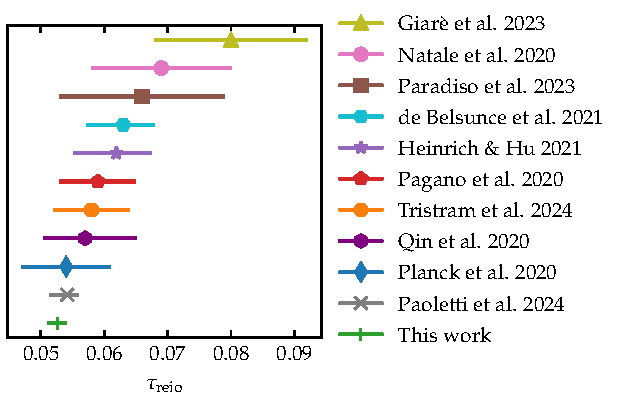
\includegraphics{figs/tau_fig.pdf}
\caption{\textbf{Current constraints on the optical depth to
reionization ($\tau_\reio$) from Cosmic Microwave Background (CMB)
data.}
The error bars indicate the 1$\sigma$ uncertainties.
Various analyses may employ distinct data sets or vary in the parameters
considered.
For instance, the inclusion of astrophysical data \cite{Qin2020,
Paoletti2024} (cross and purple hexagon), WMAP data \cite{Natale2020,
Paradiso2023} (circle and square), or ACT in combination with other
external data sets \cite{Giare2023} (triangle), expanded sky coverage
\cite{Paradiso2023} (square), incorporation of high-$\ell$ data
\cite{Pagano2020, Planck2020a, HeinrichHu2021, Giare2023, Tristram2024}
(pentagon, diamond, star, triangle, and octagon), joint low-$\ell$ TT
and EE analysis \cite{deBelsunce2021} (cyan hexagon), marginalization
over small set of strongly correlated parameters \cite{Natale2020}
(circle), and the implementation of an end-to-end Bayesian framework
that marginalizes over astrophysics and instrumental systematics
\cite{Paradiso2023} (square).}
\label{fig:tau}
\end{figure}

Given the challenges posed by $\tau_\reio$ in CMB analyses and the
anticipated advancements in constraining the reionization
timeline \cite{Montero2021, Hera2022}, now is an opportune moment to
reassess its role.
Theoretically, cosmic reionization is uniquely determined by cosmology,
i.e.\ $x_\HI(z)$ is fully determined by the other five cosmological
parameters.
However, incomplete understanding of reionization obscures this mapping,
necessitating the additional empirical parameter $\tau_\reio$ in CMB
analyses.
Since the inclusion of $\tau_\reio$ became a standard practice, our
understanding of the astrophysical processes governing reionization has
significantly improved \cite{Gnedin2022, Kannan2022,Murray2020, Fan2023}
and ongoing and forthcoming observations promise to reduce inherent
modeling uncertainties.

Motivated by these developments, we use symbolic regression (SR)
\cite{Cranmer2023, Graham2013} to construct a mapping between cosmology,
astrophysics, and reionization timeline, aiming to demote $\tau_\reio$
from an independent to a derived cosmological parameter and
simultaneously tightening constraints in cosmological and astrophysical
parameters.
This mapping can also shed light on reionization astrophysics and aid
ongoing efforts in parametrizing reionization models \cite{Trac2018,
Trac2022, Paoletti2024} by including the cosmological dependence of
$x_\HI$.

Here, we present a universality in the neutral hydrogen time evolution
related via a power-law transform, and derive through SR the
dependence of power-law parameters on cosmology and astrophysics from
simulated \texttt{21cmFAST} \cite{MesingerEtAl2011, Murray2020}
reionization histories.
We integrate this universally shaped reionization timeline into
\texttt{CLASS} \cite{Blas2011}, a popular Boltzmann solver for CMB
analyses.
We then evaluate the modified \texttt{CLASS} alongside \texttt{Cobaya}
\cite{Torrado2020}, a speed-aware sampler \cite{Lewis2002,
Lewis2013}, showcasing its ability to
recover parameter constraints from CMB data, including `TTTEEE' +
lensing likelihoods \cite{Planck2020c, Planck2020d} (see \Cref{fig:tg}).
Finally, combining CMB and astrophysical data, we marginalize over
reionization astrophysics to compute $\tau_\reio$ as a derived parameter
using SR, quantifying the gains compared to sampling over $\tau_\reio$
utilizing the conventional $\tanh$ model \cite{Lewis2008}.
We summarize our strategy in \Cref{fig:big}.

\begin{figure}[tb]
\centering
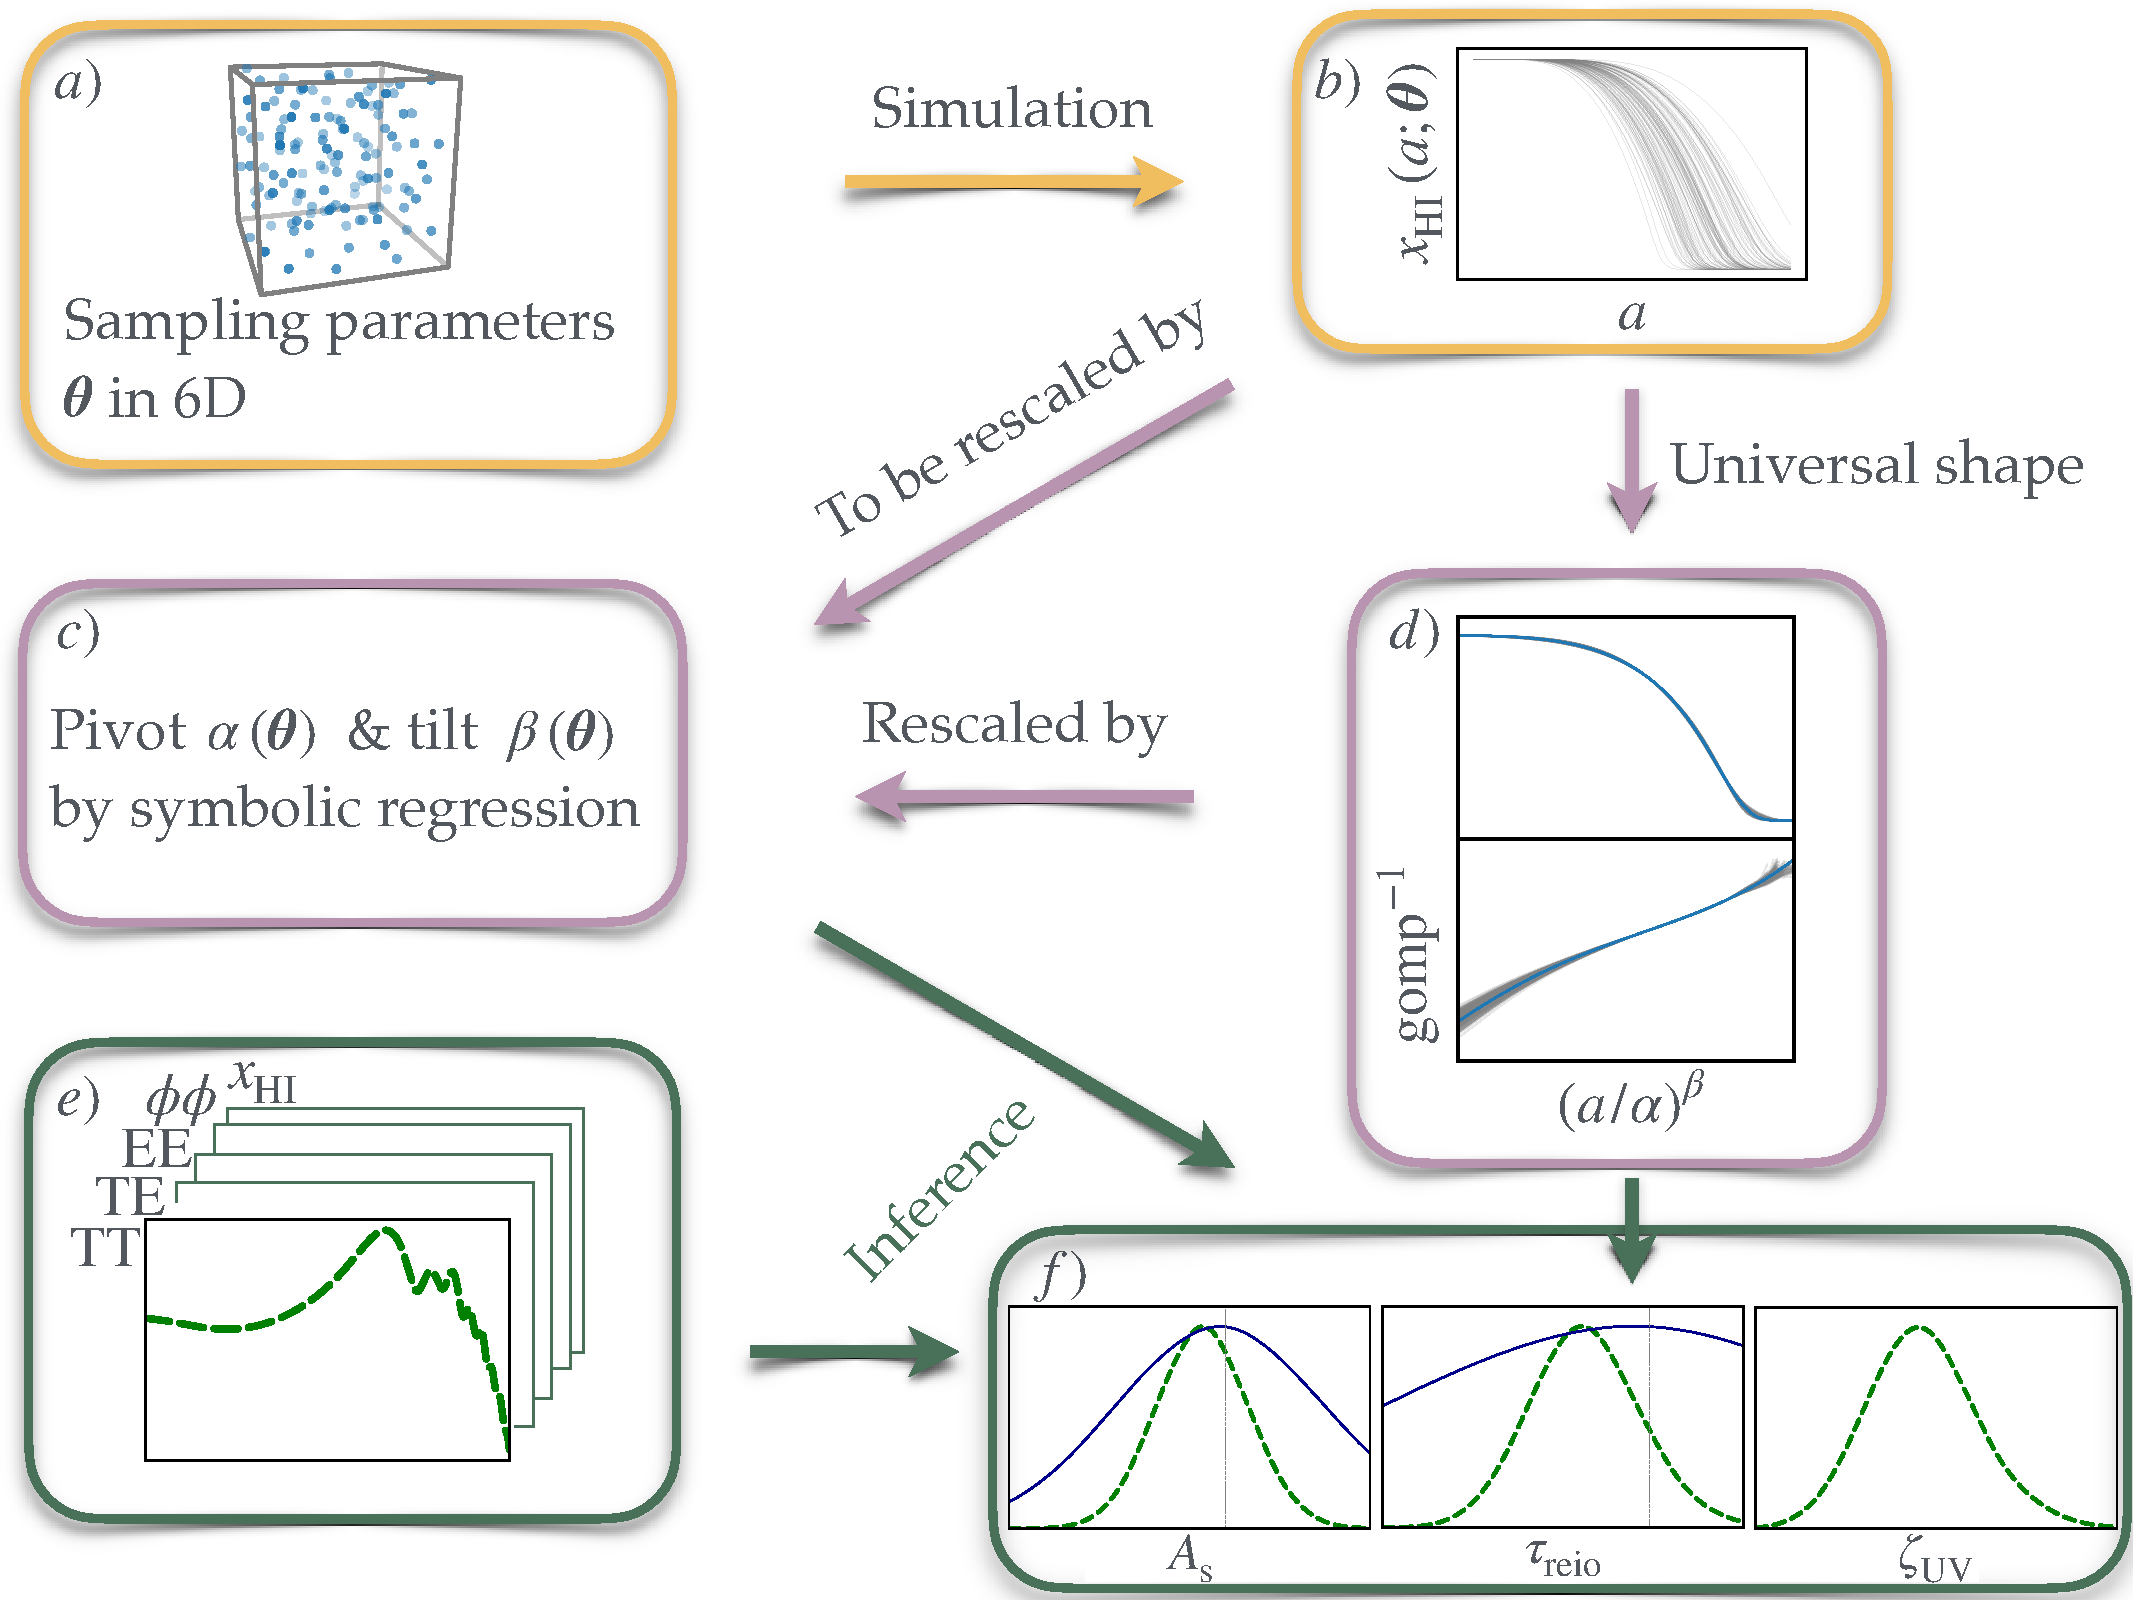
\includegraphics[width=\linewidth]{figs/big_fig.pdf}
\caption{\textbf{Strategy to demote $\tau_\reio$ to derived parameter.}
\emph{a)} Sobol sampling of $\vtheta$ comprising 5 cosmological and 1
astrophysical parameters (see \Cref{fig:sobol} in Extended Data).
\emph{b)} Simulated $x_\HI$ timelines as a function of $\vtheta$ and
scale factor $a$.
\emph{c)} With symbolic regression, we optimize the mapping from
$\vtheta$ to the rescaling parameters that bring the universality.
\emph{d)} We model the universal shape (upper panel) as a composition of
the Gompertz function and a low-degree polynomial (lower panel).
\emph{e)} Planck CMB data and $x_\HI$ data we analyze.
\emph{f)} We infer the parameter constraints using Monte Carlo Markov
Chain (MCMC).}
\label{fig:big}
\end{figure}

We construct the universal $x_\HI$ shape using 256 Sobol samples
of \texttt{21cmFAST} simulations, varying 5 cosmological parameters
and the astrophysical ionizing efficiency $\zetaUV$.
The latter modulates the timing of reionization by regulating the
abundance of photons that escape into the IGM (see \nameref{ssec:sims}
and \Cref{fig:sobol} in the Extended Data).
All $x_\HI(a)$ profiles share the same shape, with differences between
scenarios being mere translations and rescalings in logarithmic scale
factor $\ln a$.
Reionization causes $x_\HI$ to reduce from near 1 to effectively 0 via a
sigmoid transition.
The standard $\tanh$ function is symmetric in nature and not flexible
enough to provide the early start and rapid completion suggested by
reionization simulations \cite{Trac2018, Doussot2019} and favored by
astrophysical data (see \Cref{fig:history}).
In contrast, the SR-inspired Gompertz curve, an asymmetric sigmoid
function often used to analyze age-dependent human mortality
\cite{Gompertz1825}, proves a good model for the survival of neutral
hydrogen too.
Its expected accelerated increase in mortality with age resembles the
expectation for the percolation of ionized hydrogen bubbles during the
end stages of reionization.

One way to uncover the universality is to view each $x_\HI$ scenario as
a cumulative probability distribution (CDF) in $- \ln a$.
With this insight, we can translate and rescale each timeline using the
mean and variance of its corresponding probability density function
(PDF), i.e.\ $- \mathrm{d}x_\HI / \mathrm{d}\ln a$, and discover the
existence of a universal shape followed by all scenarios.
Therefore, cosmology and $\zetaUV$ only impacts the translation and
rescaling parameters of each timeline, not its shape.

However, with the PDF trick, some $x_\HI$'s can deviate artificially
from universality, due to their incomplete reionization given our broad
range of simulated scenarios.
To address this, we adopt a better approach to jointly fit the global
shape and the 2 individual parameters of each $x_\HI$.
Our shape model constitutes the Gompertz function composed with a
5th-degree polynomial, in the translated-and-rescaled time $\ln\ar
\equiv \tilt (\ln a - \ln\ap)$.
And we are free to set the polynomial constant to 0 and its linear
coefficient to 1 by utilizing their respective degeneracy with $\ln\ap$
and $\tilt$.

The complete model parametrizes the HI evolution as follows (also see
\Cref{fig:shape} and \nameref{ssec:shape} in the Extended Data):
%
\begin{align}
\label{eq:uni}
x_\HI(\ar) &= \gomp\bigl( P_5(\ar) \bigr)
  \equiv \exp\bigl[ - \exp\bigl( P_5(\ar) \bigr) \bigr], \\
%
\label{eq:poly}
P_5(\ar) &= {\textstyle\sum}_{m=0}^5 \, c_m \ln^m\!\ar, \\
%
\bm{c} &= \{0, 1, 0.1130, 0.02600, 0.0005491, -0.00006518\}, \nonumber\\
%
\label{eq:map}
\ar(a; \vtheta) &= \Bigl[ \frac{a}{\ap(\vtheta)} \Bigr]^{\tilt(\vtheta)},
\end{align}
%
where $\vtheta$ denotes 6 astrophysical and cosmological parameters,
$\ap(\vtheta)$ is the power-law pivot (or logarithmic translation), and
$\tilt(\vtheta)$ is the rescaling tilt.
Their parameter dependences stem from \texttt{21cmFAST}'s modeling of
reionization astrophysics.
Also see \nameref{ssec:helium} for specifics on implementing HeI and
HeII reionization.

Before fully leveraging our methodology to extract the parameter
dependence in the rescaling of \cref{eq:uni} and relaxing the need for
$\tau_\reio$ in CMB analyses, we first implement the Gompertz shape with
independent $\tau_\reio$ in \texttt{CLASS} and confirm its agreement
with the conventional $\tanh$ model (gomp and $\tanh$ in
\Cref{tab:uber-table}).
Using Planck PR3 likelihoods `TTTEEE' \cite{Planck2020c} and CMB lensing
\cite{Planck2020d}, we sample typical cosmological parameters with
\texttt{Cobaya} \cite{Torrado2020}, including $\tau_\reio$.
Given a proposal for $\tau_\reio$, we determine the corresponding
reionization timeline using bisection by varying $\ln\ap$ for gomp
while fixing $\beta$ to its mean value,
meanwhile for $\tanh$, the reionization midpoint $z_\re$ is the tuning
parameter.
The sampler runs until the Gelman-Rubin statistic \cite{Gelman1992}
satisfies $R - 1 < 0.01$ for the variance in parameter means from
different chains.
We repeat this for $\tanh$ and verify the agreement between the two
models.

\Cref{fig:tg,tab:uber-table} in the Extended Data summarize this
validation experiment.
The only notable differences in inferred parameters are in $z_\re$.
The gomp scenario suggests a more delayed reionization by over
$1\sigma$, with $z_\re = 6.76 \pm 0.67$ compared to $7.67 \pm 0.75$ for
$\tanh$, in alignment with recent high-$z$ quasar observations
\cite{Keating2020}.
All other cosmological parameters are in good agreement with Planck's
results \cite{Planck2020a}, with differences $\lessapprox 0.5 \%$.

Having demonstrated that the universally shaped reionization can
reproduce standard CMB analyses, we move to establish the connection
between the universal shape for $x_\HI$ and the rescaling of a given
reionization scenario.
We refer to this model as gomp + SRFull.
This rescaling naturally depends on cosmology and astrophysics.
For example, a larger matter density $\Omegam$ results in deeper
potential wells, accelerating structure formation and increasing the
number of ultraviolet photons driving the reionization process.
We employ \texttt{PySR}, an SR package, to establish the parameter
dependences of the rescaling in \cref{eq:map}.

While \texttt{PySR} initially guided us towards the Gompertz curve when
directly regressing $x_\HI$, the final analysis only uses it to regress
the pivot and tilt instead.
We fit their values jointly with the polynomial coefficients as
described above, and feed them as labels to the genetic algorithm to
find the best analytic expression (see \nameref{ssec:pysr} in Extended
Data for our definition of \emph{best}).
Using \texttt{PySR} we derived the following mapping
%
\begin{align}
\label{eq:SR_a}
\ln\ap(\vtheta) &= \Bigl(\frac{\Omegab}{\Omegam}\Bigr)^h
  - (\sigma_8 - 0.04835) \bigl(\ns + 0.3558 \ln(0.1123 \zetaUV)\bigr)
  - \Omegam - \ns, \\
%
\label{eq:SR_b}
\beta(\vtheta) &= \Bigl( \frac{0.005660^{\Omegam}}{0.6015}
    - \ln\bigl(\zetaUV - (\Omegam + \ns h)^{15.05}\bigr) + h \Bigr)
  \ln{\Omegab} + \frac{h}{\sigma_8},
\end{align}
where $\ns$, $h$, $\Omegab$, and $\Omegam$ are the tilt of the
primordial power spectrum, dimensionless Hubble constant, and present
baryon and matter density fractions, respectively.
$\sigma_8$ is the present linear rms relative density fluctuation in a
sphere of radius $8 \, h^{-1}$Mpc.

\cref{eq:map,eq:SR_a,eq:SR_b} are analytic expressions and thus
interpretable.
For example, higher values of $\Omegam$, $\sigma_8$, and $\zetaUV$
hasten reionization by enhancing structure formation and increasing the
abundance of ionizing photons.
Similarly, larger $\ns$ primarily expedites reionization by boosting
power on small scales, leading to more ionizing sources and earlier
completion \cite{Montero2021}.
Keep in mind that our \texttt{21cmFAST} simulations assume that faint
galaxies are the primary drivers of reionization.
Surprisingly, \cref{eq:SR_a,eq:SR_b} suggests that higher $\Omegab$
delays reionization, likely due to more HI in the intergalactic medium
requiring additional ionizing photons.
The ratio $\Omegab/\Omegam$ in $\alpha$ supports this view.
Moreover, increasing $h$ slightly delays reionization, consistent with
an increase in physical baryon density and
the expectation that galaxies and ionizing photons will be more spread
out.

We note that within the prior range of our \texttt{21cmFAST} simulations
(see \nameref{ssec:sims}) and their corresponding astrophysics of
reionization, the mapping derived from SR is not unique.
Additional details and results using an alternative mapping -- SRHalf --
are presented in \nameref{ssec:SRHalf} of the Extended Data.
Nonetheless, our results are robust and independent of the choice of
mapping.

We implement \cref{eq:SR_a,eq:SR_b} in our Gompertz \texttt{CLASS},
which given the cosmological and astrophysical parameters, determines
the pivot and tilt values, and consequently the reionization history,
$\tau_\reio$, and CMB angular power spectra.
This gomp + SRFull model eliminates the need to sample over $\tau_\reio$
(or $z_\re$), requiring only five cosmological parameters and $\zetaUV$.
Moreover, thanks to SR, the model can constrain $\zetaUV$ using CMB and
astrophysical data directly, a link that was not utilized in
previous efforts \cite{Greig2017}.
The advantage of sampling over $\zetaUV$ instead of $\tau_\reio$ is that
powerful astrophysical constraints on $x_\HI$ can be used to marginalize
over $\zetaUV$.
We use \texttt{Cobaya} to re-analyze the same CMB data and include
astrophysical data (see \nameref{ssec:xHI} of the Extended Data) to
effectively constrain and marginalize over $\zetaUV$.

\begin{figure}[tb]
\centering
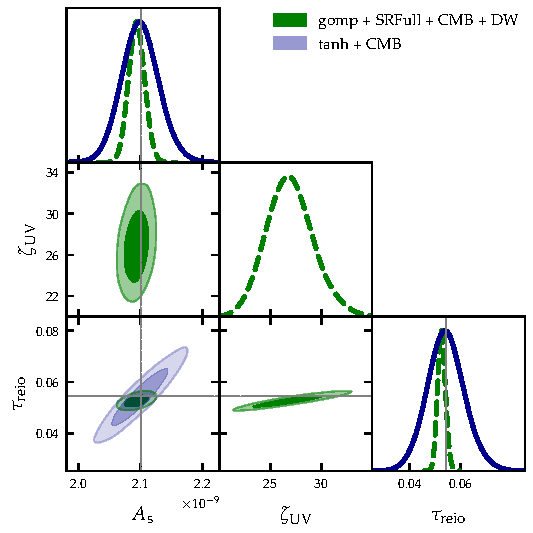
\includegraphics[width=0.7\linewidth]{figs/gomp1dw_tanh_triangle_kill.pdf}
\caption{\textbf{Analysis of CMB and astrophysical data with
reionization as a function of cosmology and astrophysics.}
The green contours represent our results using the Gompertz reionization
model with \cref{eq:SR_a,eq:SR_b}, which eliminates the need to sample
over any conventional reionization parameter and uses quasar damping
wing data on $x_\HI$ to constrain and marginalize over reionization
astrophysics.
The blue contours correspond to the results obtained using the
conventional $\tanh$ model, while the relevant Planck constraints
\cite{Planck2020a} are depicted with gray lines for reference.
The $\tanh$ model performs poorly in fitting astrophysical data; thus,
combining $\tanh$ with astrophysical data is ill-advised.}
\label{fig:kill}
\end{figure}

\Cref{fig:kill} underscores the impact of our universally-shaped
Gompertz reionization model, tightening the optical depth constraint to
$<3\%$ compared to $> 10\%$ with the $\tanh$ prescription.
Furthermore, the constraint on $\As$ improves dramatically since the TT
data is no longer significantly hampered by the degeneracy between $\As$
and $\tau_\reio$.
The error on $\As$ decreases by an impressive factor of 2.3 compared to
Planck's results \cite{Planck2020a}.
Overall, we recover tighter constraints across the board compared to
Planck.
Notably, combining SR with CMB and astrophysical data, specifically
quasar damping wing (DW) data, yields a highly competitive constraint on
$\zetaUV = 26.9^{+2.1}_{-2.5}$, a commanding improvement over previous
constraints (e.g.\ $\zetaUV = 28^{+52}_{-18}$) \cite{Greig2017}.
See \nameref{ssec:fits}, \Cref{fig:unleashed_gomp,tab:uber-table} in the
Extended Data for details.

\begin{figure}[tb]
\centering
\includegraphics[width=0.66\linewidth]{figs/history.pdf}
\caption{\textbf{Optical depth evolution $\tau(z)$ and reionization
history $x_\HI(z)$.}
Our best-fit gomp + SRFull model (green dotted line) of Planck CMB data
+ quasar damping wing (DW) data is asymmetric and differs significantly
from that of the symmetric $\tanh$ model (blue solid line).
Note $z$ is shown in logarithmic scale of $a^{-1}$.
We also include an alternative mapping from physical parameters to
Gompertz timeline -- gomp + SRHalf -- in the purple dashed line (see
\nameref{ssec:SRHalf}).
The shaded regions in the upper panel correspond to the inferred range
in $\tau_\reio$ from analyzing Planck PR3 data.
Additionally, the lower panel includes observational constraints from
high-redshift quasars and galaxies (see \nameref{ssec:xHI}).}
\label{fig:history} \end{figure}

Our results suggest that Planck data favors a delayed reionization
compared to other CMB-based constraints (in a $\chi^2$-sense).
Our best-fit cosmological parameters indicate a midpoint of $z_\re =
6.98$ and a duration of $\Delta z \equiv z(x_\HI = 0.05) - z(x_\HI =
0.95) \approx 560 $ Myr, consistent with our previous constraint
without SR.
While our results align with late reionization observations, the
difference from $\tanh$ is within 1$\sigma$.
The duration of reionization, though better suited to observational
constraints compared to $\tanh$, might still be considered somewhat
rapid in the context of late reionization scenarios \cite{Cain2021}.
\Cref{fig:history} illustrates the reionization timeline derived from
our best-fit values, in contrast with the poor fit of symmetric $\tanh$
to the astrophysical data.

Our findings for the timeline of reionization align with late
reionization scenarios, which are supported by high-$z$ Lyman-$\alpha$
observations \cite{Keating2020, Cain2021}.
However, recent discoveries by JWST indicate the presence of massive,
bright galaxies at early redshifts $z \sim 10$ \cite{Adams2023,
Bradley2023, Donnan2023}.
The presence of these early galaxies suggests a potential preference for
brighter galaxies to drive reionization, a role that in our
\texttt{21cmFAST} simulations was attributed to a population of faint
galaxies.

We note that our results assume a flat Universe.
Relaxing this assumption requires adding an extra parameter to the
functional form of $\tau$ \cite{Anselmi2023}.
Furthermore, our results are influenced by the semi-numerical
prescription employed by \texttt{21cmFAST} to ionize the IGM, which,
while efficient and swift, could bias our findings.
Moreover, our exploration within the astrophysical framework of
\texttt{21cmFAST} has been limited to varying the ionization efficiency
(see \nameref{ssec:sims} in the Extended Data).
Therefore, a more comprehensive exploration is warranted to ensure, for
instance, that our findings for $\alpha$ and $\beta$ will not bias
cosmological analyses when incorporating additional astrophysical
parameters, such as the minimum halo mass that host ionizing sources.
Additionally, a valuable exercise to refine the inherent relationship
between cosmological parameters and reionization history would involve
using more realistic, albeit slower, reionization models.
One such option is to use the THESAN simulations \cite{Kannan2022},
which are hydrodynamical simulations incorporating radiative transfer.

Throughout this work we considered only DW for astrophysical data,
but including current luminosity function constraints can already halve
the error on $\tau_\reio$.
Hence, as reionization constraints improve, we anticipate substantial
cosmological gains with our framework.
